%%%%%%%%%%%%%%%%%%%%%%%%%%%%%%%%%%%%%%%%%
% Beamer Presentation
% LaTeX Template
% Version 1.0 (10/11/12)
%
% This template has been downloaded from:
% http://www.LaTeXTemplates.com
%
% License:
% CC BY-NC-SA 3.0 (http://creativecommons.org/licenses/by-nc-sa/3.0/)
%
%%%%%%%%%%%%%%%%%%%%%%%%%%%%%%%%%%%%%%%%%

%----------------------------------------------------------------------------------------
%	PACKAGES AND THEMES
%----------------------------------------------------------------------------------------

\documentclass[xcolor=svgnames]{beamer}

\mode<presentation> {

% The Beamer class comes with a number of default slide themes
% which change the colors and layouts of slides. Below this is a list
% of all the themes, uncomment each in turn to see what they look like.

% \usetheme{default}
% \usetheme{AnnArbor}
% \usetheme{Antibes}
%\usetheme{Bergen}
% \usetheme{Berkeley}
% \usetheme{Berlin}
\usetheme{Boadilla}
% \usetheme{CambridgeUS}
% \usetheme{Copenhagen}
% \usetheme{Darmstadt}
% \usetheme{Dresden}
% \usetheme{Frankfurt}
% \usetheme{Goettingen}
% \usetheme{Hannover}
% \usetheme{Ilmenau}
% \usetheme{JuanLesPins}
% \usetheme{Luebeck}
% \usetheme{Madrid}
% \usetheme{Malmoe}
% \usetheme{Marburg}
% \usetheme{Montpellier}
% \usetheme{PaloAlto}
% \usetheme{Pittsburgh}
% \usetheme{Rochester}
% \usetheme{Singapore}
% \usetheme{Szeged}
% \usetheme{Warsaw}

% As well as themes, the Beamer class has a number of color themes
% for any slide theme. Uncomment each of these in turn to see how it
% changes the colors of your current slide theme.

% \usecolortheme{albatross}
% \usecolortheme{beaver}
%\usecolortheme{beetle}
% \usecolortheme{crane}
%  \usecolortheme{dolphin}
% \usecolortheme{dove}
% \usecolortheme{fly}
% \usecolortheme{lily}
% \usecolortheme{orchid}
% \usecolortheme{rose}
% \usecolortheme{seagull}
% \usecolortheme{seahorse}
% \usecolortheme{whale}
% \usecolortheme{wolverine}

% \setbeamertemplate{footline} % To remove the footer line in all slides uncomment this line
%\setbeamertemplate{footline}[page number] % To replace the footer line in all slides with a simple slide count uncomment this line

% \setbeamertemplate{navigation symbols}{} % To remove the navigation symbols from the bottom of all slides uncomment this line
}

\usepackage{graphicx} % Allows including images
\usepackage{booktabs} % Allows the use of \toprule, \midrule and \bottomrule in tables
\usepackage{tikz}
\usepackage{multicol}
\usepackage{wrapfig}
\usepackage{amsmath,amsthm,amssymb}
\usepackage{mathtools}
\usepackage{multicol}
\usepackage{hyperref}
\DeclarePairedDelimiter\ceil{\lceil}{\rceil}
\DeclarePairedDelimiter\floor{\lfloor}{\rfloor}


\addtobeamertemplate{frametitle}{}{%
\begin{tikzpicture}[remember picture,overlay]
\node[anchor=north east,yshift=2pt] at (current page.north east) {
\includegraphics[height=0.8cm]{iiit-new.png}};
\end{tikzpicture}}

\setbeamercolor{title in head/foot}{bg=OrangeRed, fg=White}
\setbeamercolor{author in head/foot}{bg=RoyalBlue, fg=White}
\setbeamercolor{date in head/foot}{bg=SlateGray, fg=Black}

%----------------------------------------------------------------------------------------
%	TITLE PAGE
%----------------------------------------------------------------------------------------

\title[Discrete Structures]{Discrete Structures} % The short title appears at the bottom of every slide, the full title is only on the title page
\author{IIIT Hyderabad} % Your name
\institute[] % Your institution as it will appear on the bottom of every slide, may be shorthand to save space
{
Monsoon 2020 \\ % Your institution for the title page
\medskip
\textit{Tutorial 10} % Your email address
}
\date{October 19 , 2020} % Date, can be changed to a custom date
\newcommand{\comment}[1]{}
\begin{document}

\begin{frame}
\titlepage % Print the title page as the first slide
\end{frame}

\begin{frame}
\frametitle{Introduction} % Table of contents slide, comment this block out to remove it
\tableofcontents % Throughout your presentation, if you choose to use \section{} and \subsection{} commands, these will automatically be printed on this slide as an overview of your presentation
\end{frame}

%----------------------------------------------------------------------------------------
%	PRESENTATION SLIDES
%----------------------------------------------------------------------------------------

%------------------------------------------------
\section{Questions}
%------------------------------------------------

%------------------------------------------------
\subsection{Question 1}
%------------------------------------------------

\begin{frame}
    Prove the following -
    \begin{enumerate}
    \item A function $f$ has left inverse $\iff$ it is injective.
    \\ \textbf{Sol:} Say $f:A \rightarrow B$
    
    $\implies$ part :
    
    Suppose $f$ has a left inverse, we need to show that it is injective, that is 
    \begin{align}
    f(x_1) = f(x_2) \implies x_1 = x_2
    \end{align}
    Assume $f(x_1) = f(x_2)$. We shall prove $x_1 = x_2$. Say, if  $g$ is the left inverse of it, then we have 
    \begin{align}
        g(f(x_1)) &= x_1 & \ldots \text{ \{definition of left inverse\}}
        \\ g(f(x_2)) &= x_2 & \ldots \text{ \{definition of left inverse\}}
        \\g(f(x_1)) &= g(f(x_2)) & \ldots \text{ \{as $f(x_1)  = f(x_2)$\}}
        \\ x_1 &= x_2 & \ldots \text{ \{from (2) and (3)\}}
    \end{align}
\end{enumerate}

\end{frame}

\begin{frame}{}
\footnotesize{
    $\impliedby$ part:
    Construct $g:B \rightarrow A$ such that - 
    \begin{align*}
    g(y) &= 
        \begin{cases}
        x \text{ if $\exists x, f(x) = y$}
        \\ c \text{ otherwise}
        \end{cases}
    \end{align*}
    Here $c$ is an arbitary fixed element $\in A$. 
    We need to prove that it is a function, in order to do that, we need to prove that it is 
    \begin{enumerate}
        \item Exhaustive over domain. That is $\forall y \in B, g(y)$ is defined. This is true by our construction (either an element will have it's pre-image or will be mapped to the element $c$).
        \item $\forall y \in B, (g(y) = x_1) \land (g(y) = x_2) \implies x_1 = x_2$. Say if this were not true, we have that $g(y) = x_1$ and $g(y) = x_2$ but $x_1 \neq x_2$. Either of the 2 cases can happen - 
        \begin{enumerate}
            \item $y$ doesn't have a pre-image in A. In which case both $x_1,x_2$ must be equal to $c$. That is, $x_1 = x_2 = c$.
            \item $y$ has a pre-image in A, thus $x_1$ and $x_2$ are 2 distinct pre-images of $y$. Or $f(x_1) = f(x_2) = y$. but since $f$ is injective, we must have $x_1 = x_2$.
        \end{enumerate}
    \end{enumerate}
    Thus $g$ should be a function.Now we have 
    \begin{align*}
        & (\forall x \in A) \text{ } g \circ f(x) 
        \\ &= g(y) & \ldots \text{\{where $y = f(x)$\}}
        \\ &= x & \ldots \text{\{ by definition\}}
    \end{align*}
    Thus we have $g$ is indeed a left-inverse function.
}
\end{frame}

\begin{frame}{}
    \begin{enumerate}\setcounter{enumi}{1}
        \item A function $f$ has right inverse $\iff$ it is surjective.
    \\ \textbf{Sol:} 
    
    $\implies$ part:
    
    Suppose $f$ has a right inverse, say $g$. For surjectivity, we need to show that 
    \begin{align*}
     (\forall y \in B)  (\exists x \in A, f(x) = y)
    \end{align*}
    
    For any $y \in B$, take $x = g(y)$ (this we can take since $g$ is a function), indeed we have 
    \begin{align*}
        f(x) &= f \circ g(y) &
        \\ &= y & \ldots \text{\{ by definition of right inverse.\}}
    \end{align*}
    Thus for any $y$, we have it's pre-image as $x = g(y)$. Thus the function $f$ is surjective.
    \end{enumerate}

\end{frame}

\begin{frame}{}
\footnotesize{$\impliedby$ part:

Now if, $f$ is surjective, construct a mapping $g:B \rightarrow A$. Since $f$ is surjective, and for each $y$, we have atleast one pre-images. Let's say we map it to only one of them -
\begin{align*}
 \forall y \in B, g(y) = x \text{ such that } f(x) = y 
\end{align*}
  The function $g$ is 
  \begin{enumerate}
      \item Exhaustive over domain. That is $\forall y \in B, g(y)$ is defined. This is true by our construction (we are defining it over all $y \in B$).
        \item $\forall y \in B, (g(y) = x_1) \land (g(y) = x_2) \implies x_1 = x_2$. Since we are choosing only one of the pre-images, an element will never be mapped to more than 1 distinct pre-image.
  \end{enumerate}
Thus $g$ is a function, indeed - 
\begin{align*}
    & f \circ g(y) &
    \\ &= f (x) & \ldots \text{ \{ where $f(x) = y$, by construction \}}
    \\ &= y
\end{align*}
Thus our function is right inverse.
}
\end{frame}
\begin{frame}{}
    \begin{enumerate}\setcounter{enumi}{2}
    \item Prove that f is onto $\iff h \circ f(x) = k \circ f(x) $ implies $h=k$. 
    \\ \textbf{Sol:} 
    
    $\implies$ part:
    Since $f$ is onto, 
    \begin{align*}
        \forall y \in B, \exists x \in A \rightarrow f(x) = y
    \end{align*}
    Thus we have, 
    \begin{align*}
        h(y) & &
        \\ &= h(f(x)) & \ldots \text{\{ pre-image $x$ exists\}}
        \\ &= k(f(x)) & \ldots \text{\{ assumption\}}
        \\ &= k(y)& \ldots \text{\{ y = $f(x)$\}}
    \end{align*}
    Thus we get, $\forall y \in B, h(y) = k(y)$. Hence they are same.
\end{enumerate}

\end{frame}


%------------------------------------------------
\subsection{Question 2}
%------------------------------------------------

\begin{frame}{Question 2}
    \textbf{2.1:} Prove that the set of of all odd numbers are countable.
    \\ \textbf{Sol:} We construct a mapping - 
    \begin{align*}
        1 &\rightarrow 1
        \\ 3 &\rightarrow 2
        \\ 5 &\rightarrow 3
        \\ \vdots 
    \end{align*}
    The function can be written as $f(n) = \frac{n + 1}{2}$. It can be seen that this is a injective function as $f(n_1) = f(n_2) \implies n_1 = n_2$. And that this function is surjective, as we are able  to list out each and every $n \in \mathbb{N}$ in the set. Thus it is bijective.
\end{frame}

\begin{frame}{}
    \\ \textbf{2.2:} Prove that $\mathbb{Z} \times \mathbb{Z}$ is countable.
    \\ \textbf{Sol:} We construct a mapping - 
    
    \begin{multicols}{2}
    \begin{align*}
        (0,0) &\rightarrow 1
        \\ (1,0) &\rightarrow 2
        \\ (0,1) &\rightarrow 3
        \\ (-1,0) & \rightarrow 4
        \\ (0,-1) &\rightarrow 5
        \\ (2,0) &\rightarrow 6
        \\ \vdots
    \end{align*}
    \begin{center}
        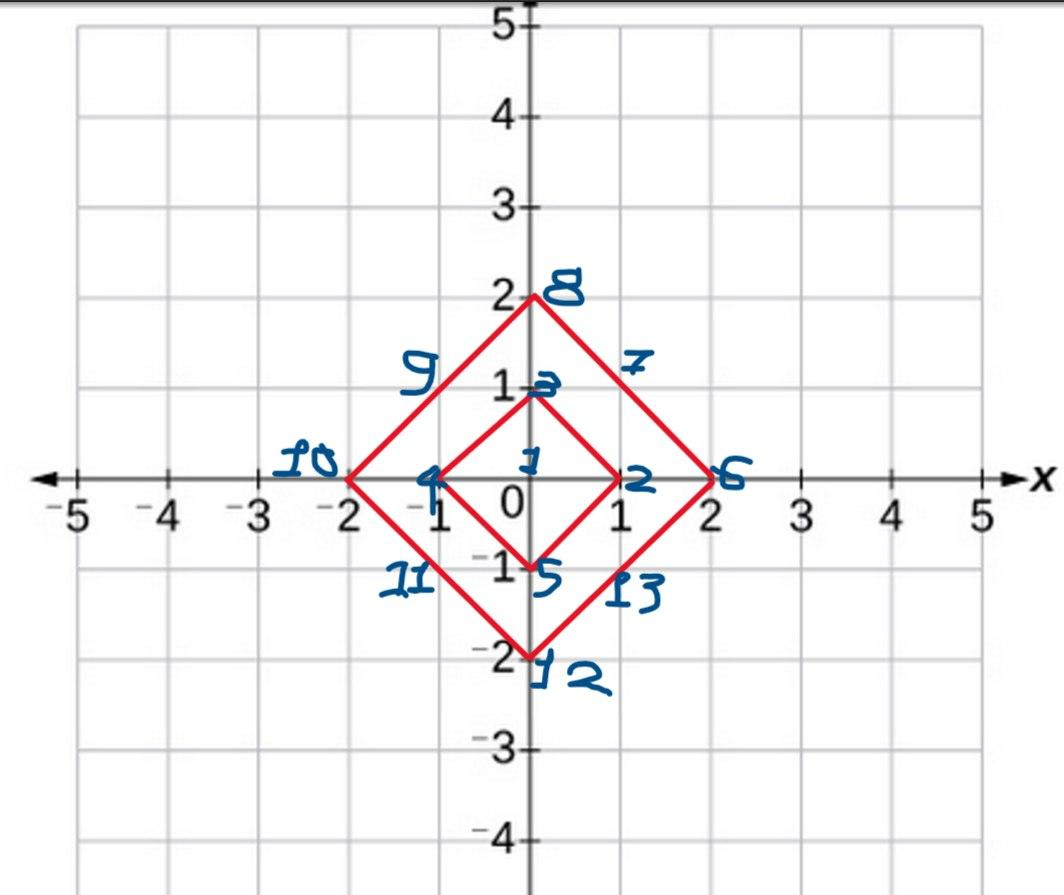
\includegraphics[width=1.2\linewidth]{photo_2020-10-20_10-20-57.jpg}
    \end{center}
    \end{multicols}
    We claim this mapping is injective, as it map's to all elements uniquely (no natural number is repeated). This mapping is surjective as we are listing out all the natural numbers one by one, and hence all numbers are listed.
\end{frame}

\end{document} 